\documentclass{standalone}
\usepackage{tikz}
\usepackage{ctex,siunitx,upgreek}
\setCJKmainfont{Noto Serif CJK SC}
\usepackage{tkz-euclide}
\usepackage{amsmath,amssymb}
\DeclareMathOperator{\arccot}{arccot}
\usetikzlibrary{patterns, calc,3d}
\usetikzlibrary {decorations.pathmorphing,decorations.pathreplacing,decorations.shapes}
\begin{document}
\small
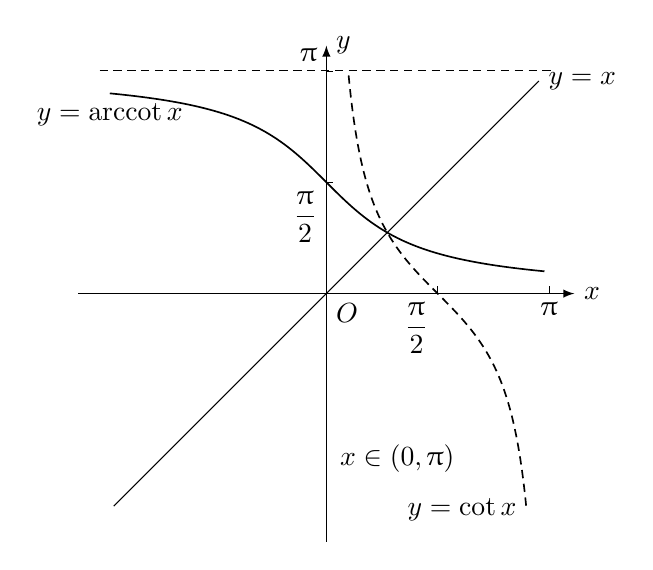
\begin{tikzpicture}[>=latex,scale=0.9]
  \draw[->](-3.5,0)--(3.5,0)node[right]{$x$};
  \draw[->](0,-3.5)--(0,3.5)node[right]{$y$};
  \node at (0,0)[below right]{$O$};
  \draw[semithick,samples=200,domain=0.1*pi:0.9*pi] plot ({cot(\x r)},\x)node[below]{$y=\arccot x$};
  \draw[semithick,densely dashed,samples=200,domain=0.1*pi:0.9*pi] plot (\x,{cot(\x r)})node[left]{$y=\cot x$};
  \draw(-3,-3)--(3,3)node[right]{$y=x$};
  \draw[densely dashed](-3.2,pi)--(3.2,pi);
  \draw[very thin](pi,0)node[below]{$\uppi$}--++(0,0.1);
  \draw[very thin](0.5*pi,0)node[below left]{$\dfrac\uppi2$}--++(0,0.1);
  \draw[very thin](0,pi)node[above left]{$\uppi$}--++(0.1,0);
  \draw[very thin](0,0.5*pi)node[below left]{$\dfrac\uppi2$}--++(0.1,0);
  \node at (1.0,-2.0)[below]{$x\in(0,\uppi)$};
\end{tikzpicture}
\end{document}